\documentclass{article}

\usepackage{enumitem}
\usepackage{listings}
\usepackage{graphicx}
\usepackage{float}
\usepackage{subcaption}
\usepackage{mwe}

\usepackage{color} %red, green, blue, yellow, cyan, magenta, black, white
\definecolor{mygreen}{RGB}{28,172,0} % color values Red, Green, Blue
\definecolor{mylilas}{RGB}{170,55,241}
\usepackage{float}
\usepackage{hyperref}

\title{CS5487 Programming Assignment 1}
\date{2019 October}
\author{Ji Yang}

\begin{document}
\maketitle

\lstset{language=Matlab,%
    %basicstyle=\color{red},
    breaklines=true,%
    morekeywords={matlab2tikz},
    keywordstyle=\color{blue},%
    morekeywords=[2]{1}, keywordstyle=[2]{\color{black}},
    identifierstyle=\color{black},%
    stringstyle=\color{mylilas},
    commentstyle=\color{mygreen},%
    showstringspaces=false,%without this there will be a symbol in the places where there is a space
    numbers=left,%
    numberstyle={\tiny \color{black}},% size of the numbers
    numbersep=9pt, % this defines how far the numbers are from the text
    emph=[1]{for,end,break},emphstyle=[1]\color{red}, %some words to emphasise
    %emph=[2]{word1,word2}, emphstyle=[2]{style},    
}

\section*{Polynomial Function}
\subsection*{(a) Implement 5 regression algorithms}
Source code can be found at \url{https://github.com/yangji12138/machine-learning/tree/master/Programming%201} or the Codes Appendix.

\subsection*{(b) Using Sample Data to estimate 5-th order poly function}

\begin{table}[H]
    \begin{tabular}{|c|c|c|c}
    \hline
        & Least-Sqaures (LS)     & \begin{tabular}[c]{@{}c@{}}Regularized LS (RLS)\\ $\lambda$ = 0.48\end{tabular} & \multicolumn{1}{c|}{\begin{tabular}[c]{@{}c@{}}L1-Regularized LS (LASSO)\\ $\lambda$ = 0 \end{tabular}} \\ \hline
    MSE & 0.4086                 & 0.4076                                                                       & \multicolumn{1}{c|}{0.4086}                                                                            \\ \hline
        & Robust Regression (RR) & Bayesian Regression (BR)                                                     &                                                                                                        \\ \cline{1-3}
    MSE & 0.7680                 & 0.4592                                                                       &                                                                                                        \\ \cline{1-3}
    \end{tabular}
\end{table}

\begin{figure}[H]
    \centering
    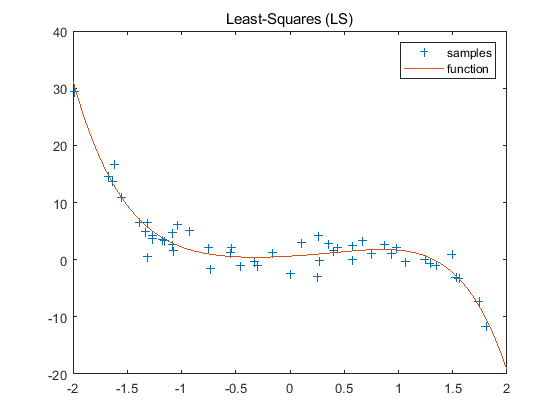
\includegraphics[width=0.75\textwidth]{fig/1b-ls.png}
    \label{fig:1b-ls}
\end{figure}

\begin{figure}
    \centering
    \begin{subfigure}[b]{0.475\textwidth}
        \centering
        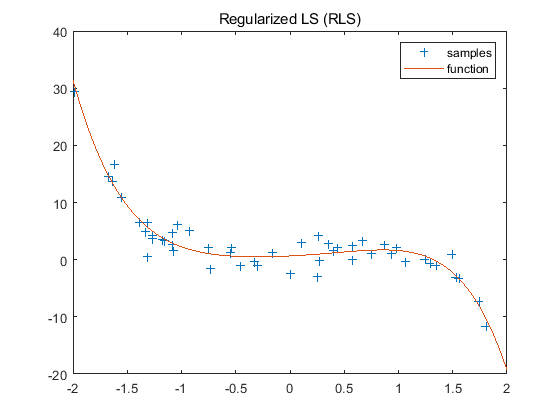
\includegraphics[width=\textwidth]{fig/1b-rls.png} 
    \end{subfigure}
    \hfill
    \begin{subfigure}[b]{0.475\textwidth}  
        \centering 
        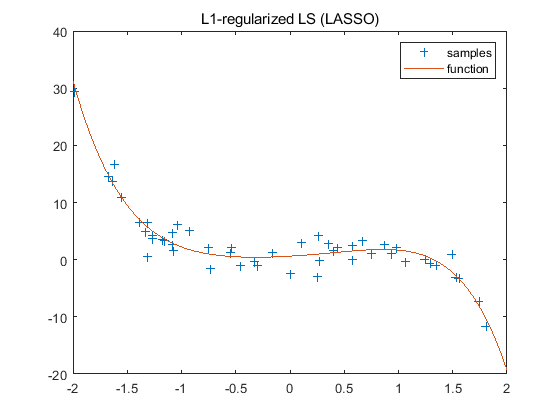
\includegraphics[width=\textwidth]{fig/1b-lasso.png}   
    \end{subfigure}
    \vskip\baselineskip
    \begin{subfigure}[b]{0.475\textwidth}   
        \centering 
        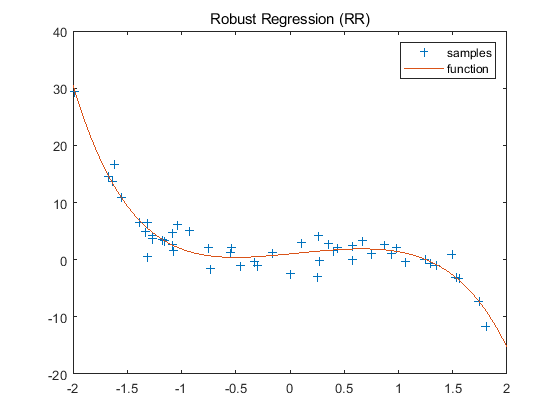
\includegraphics[width=\textwidth]{fig/1b-rr.png} 
    \end{subfigure}
    \quad
    \begin{subfigure}[b]{0.475\textwidth}   
        \centering 
        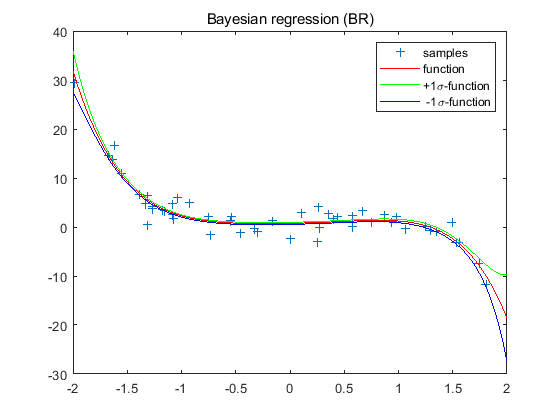
\includegraphics[width=\textwidth]{fig/1b-br.png} 
    \end{subfigure}
\end{figure}

\subsection*{(c) Subset of Training Data}

\begin{table}[H]
    \centering
    \begin{tabular}{|c|c|c|c|c}
    \hline
        & \begin{tabular}[c]{@{}c@{}}Subset \\ Ratio\end{tabular} & Least-Sqaures (LS)     & \begin{tabular}[c]{@{}c@{}}Regularized LS (RLS)\\ $\lambda$ = 0.48\end{tabular} & \multicolumn{1}{c|}{\begin{tabular}[c]{@{}c@{}}L1-Regularized LS (LASSO)\\ $\lambda$ = 0.5\end{tabular}} \\ \hline
    MSE & 10\%                                                    & 28.312                 & 82.205                                                                       & \multicolumn{1}{c|}{27.046}                                                                           \\ \hline
        & 25\%                                                    & 10.793                 & 3.475                                                                        & \multicolumn{1}{c|}{1.138}                                                                            \\ \hline
        & 50\%                                                    & 12.857                 & 0.284                                                                        & \multicolumn{1}{c|}{0.95}                                                                             \\ \hline
        & 75\%                                                    & 0.332                  & 0.941                                                                        & \multicolumn{1}{c|}{0.563}                                                                            \\ \hline
        &                                                         & Robust Regression (RR) & Bayesian Regression (BR)                                                     &                                                                                                       \\ \cline{1-4}
    MSE & 10\%                                                    & 13069.7                & 31.689                                                                       &                                                                                                       \\ \cline{1-4}
        & 25\%                                                    & 1.011                  & 13.292                                                                       &                                                                                                       \\ \cline{1-4}
        & 50\%                                                    & 3.95                   & 0.307                                                                        &                                                                                                       \\ \cline{1-4}
        & 75\%                                                    & 0.257                  & 0.73                                                                         &                                                                                                       \\ \cline{1-4}
    \end{tabular}
    \end{table}

\begin{figure}
    \centering
    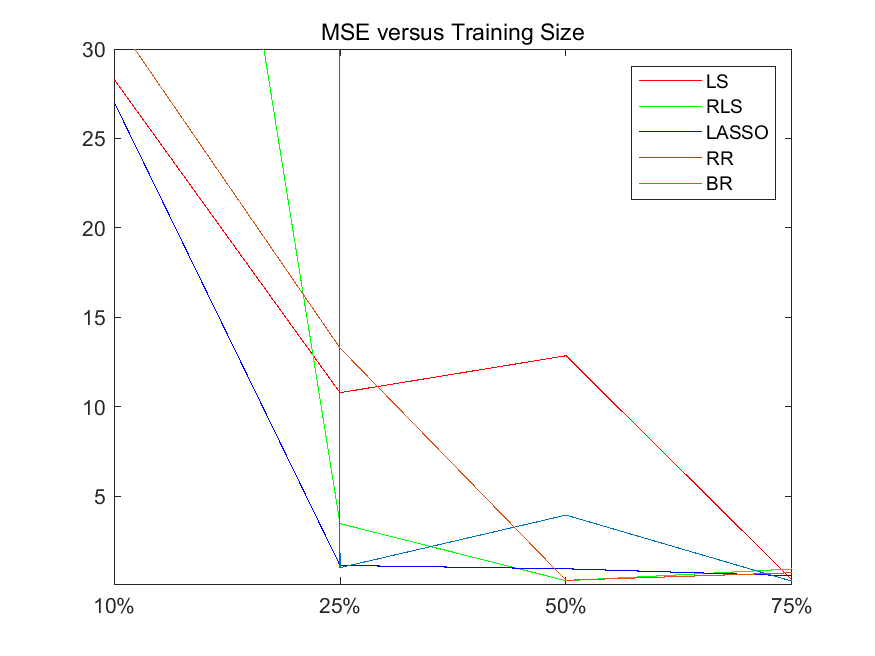
\includegraphics[width=0.45\textwidth]{fig/1c-error.png} 
    \caption{MSE versus training set}
\end{figure}

\begin{figure}[H]
        \centering
        \begin{subfigure}[b]{0.475\textwidth}
            \centering
            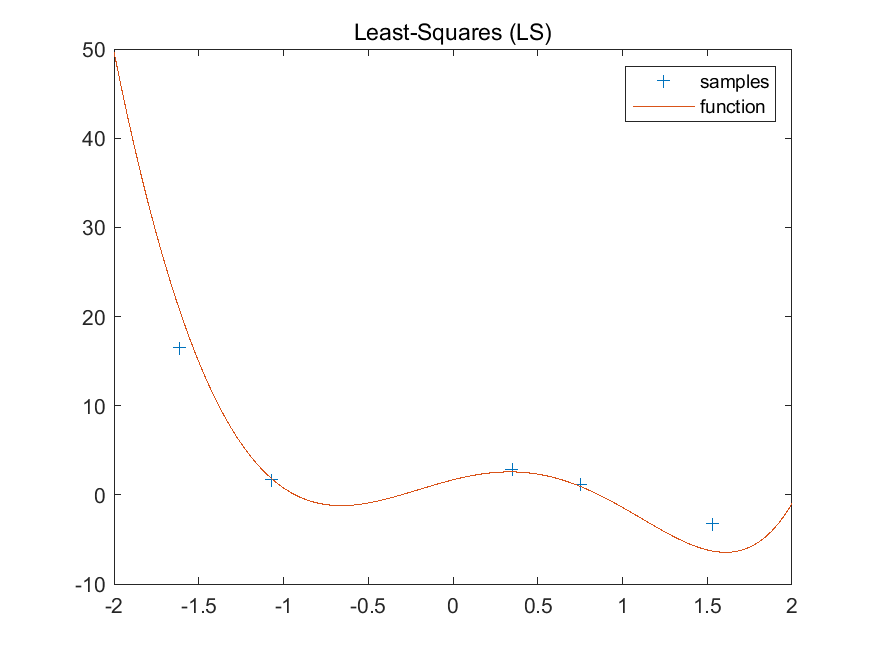
\includegraphics[width=\textwidth]{fig/1c-10-ls.png} 
        \end{subfigure}        
        \vskip\baselineskip
        \begin{subfigure}[b]{0.475\textwidth}
            \centering
            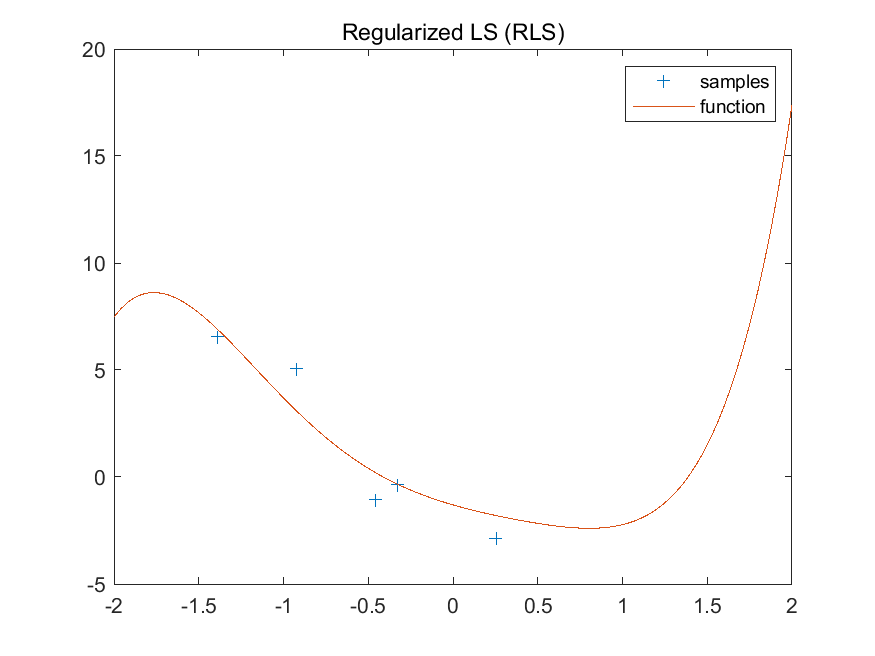
\includegraphics[width=\textwidth]{fig/1c-10-rls.png} 
        \end{subfigure}
        \hfill
        \begin{subfigure}[b]{0.475\textwidth}  
            \centering 
            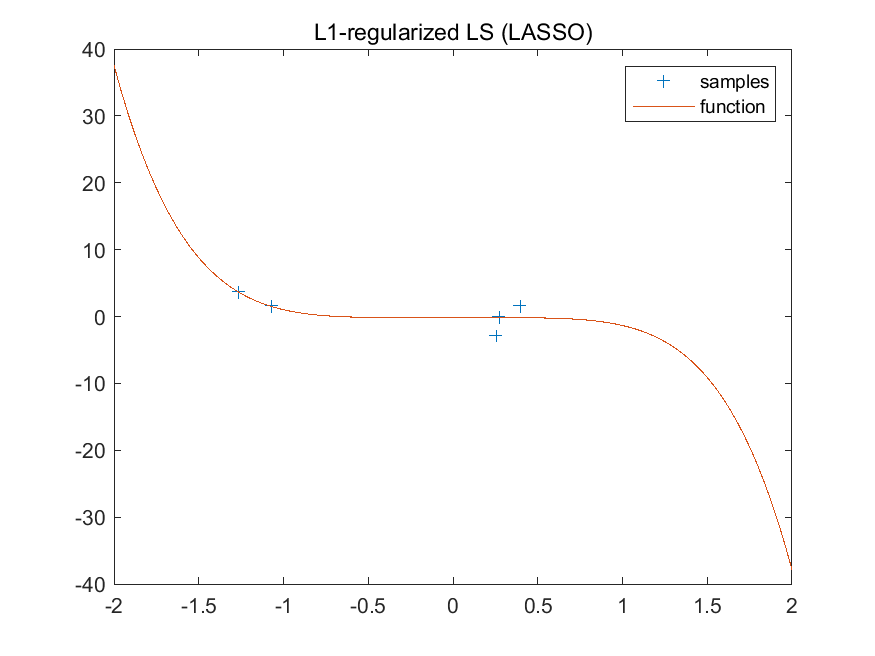
\includegraphics[width=\textwidth]{fig/1c-10-lasso.png}   
        \end{subfigure}
        \vskip\baselineskip
        \begin{subfigure}[b]{0.475\textwidth}   
            \centering 
            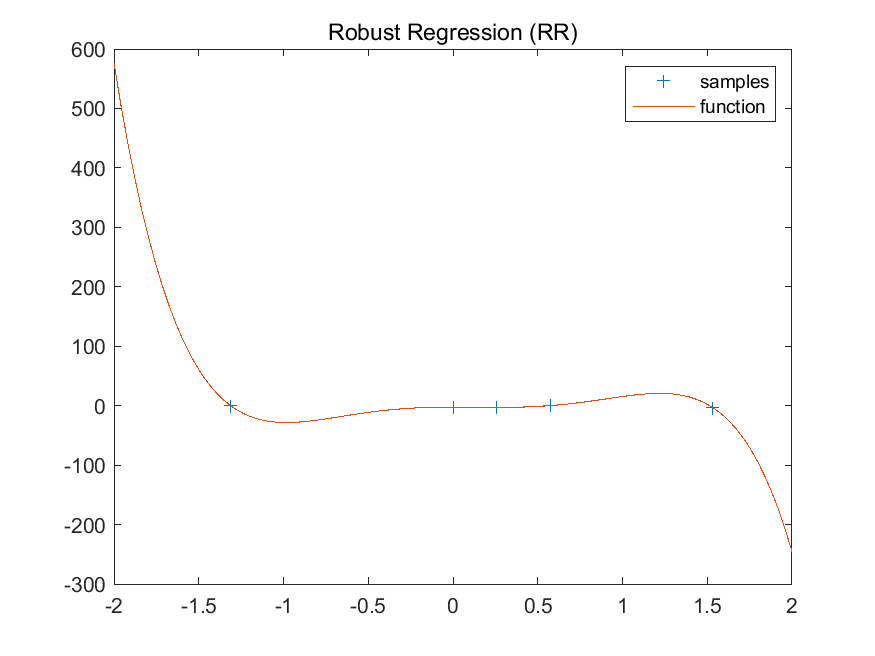
\includegraphics[width=\textwidth]{fig/1c-10-rr.png} 
        \end{subfigure}
        \quad
        \begin{subfigure}[b]{0.475\textwidth}   
            \centering 
            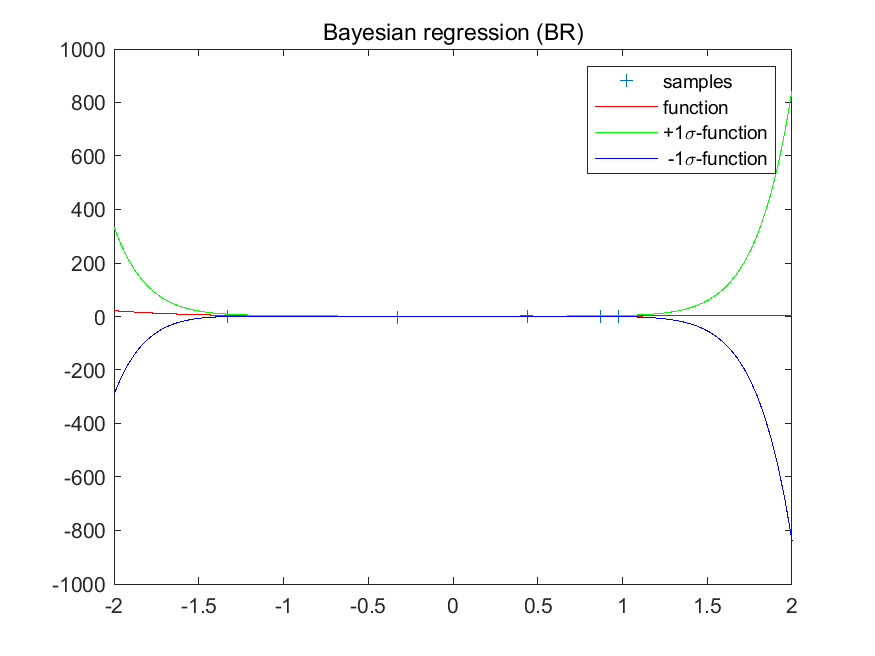
\includegraphics[width=\textwidth]{fig/1c-10-br.png} 
        \end{subfigure}
        \caption{10\% Random Sample}
\end{figure}

\begin{figure}[H]
    \centering
    \begin{subfigure}[b]{0.475\textwidth}
        \centering
        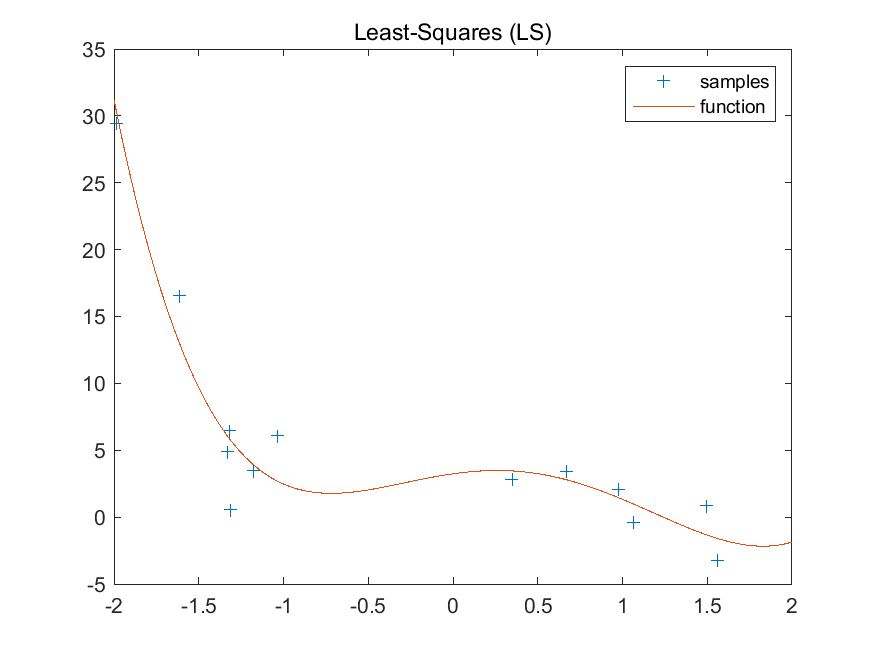
\includegraphics[width=\textwidth]{fig/1c-25-ls.png} 
    \end{subfigure}        
    \vskip\baselineskip
    \begin{subfigure}[b]{0.475\textwidth}
        \centering
        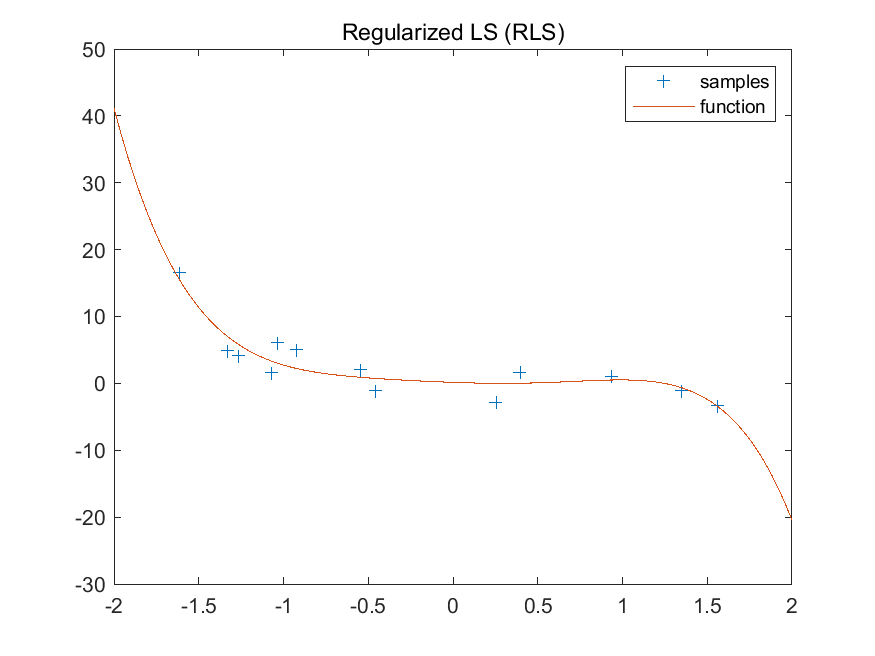
\includegraphics[width=\textwidth]{fig/1c-25-rls.png} 
    \end{subfigure}
    \hfill
    \begin{subfigure}[b]{0.475\textwidth}  
        \centering 
        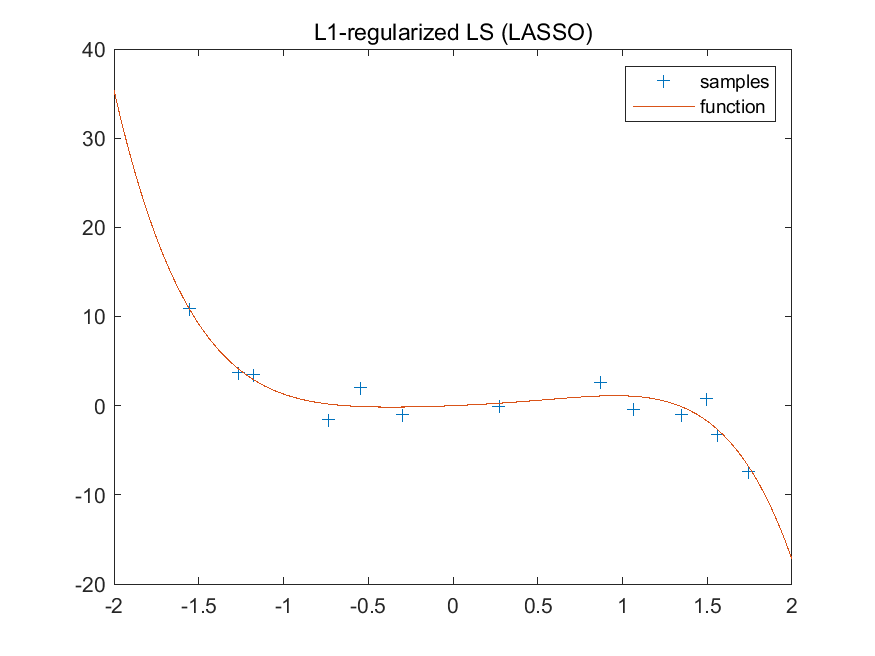
\includegraphics[width=\textwidth]{fig/1c-25-lasso.png}   
    \end{subfigure}
    \vskip\baselineskip
    \begin{subfigure}[b]{0.475\textwidth}   
        \centering 
        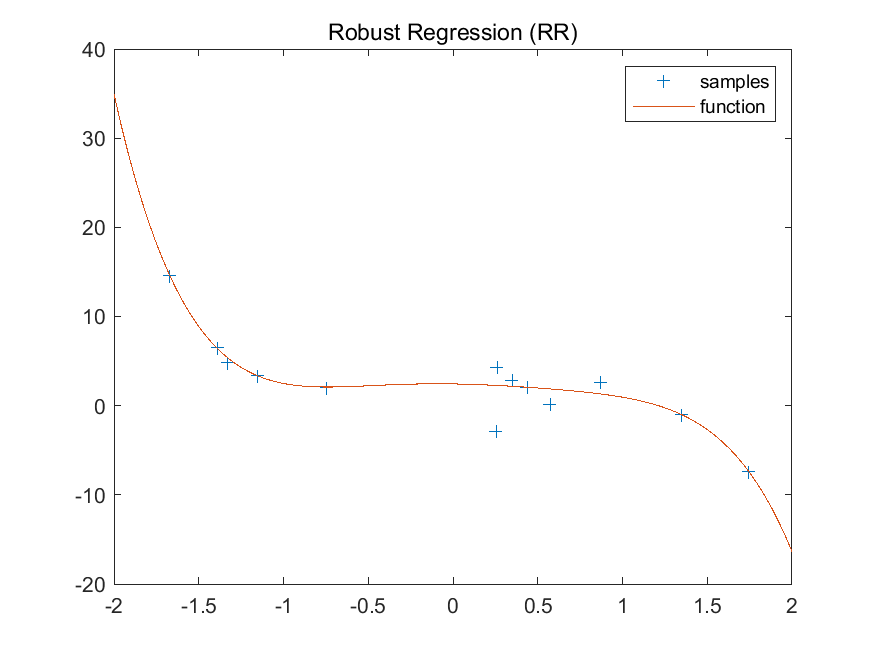
\includegraphics[width=\textwidth]{fig/1c-25-rr.png} 
    \end{subfigure}
    \quad
    \begin{subfigure}[b]{0.475\textwidth}   
        \centering 
        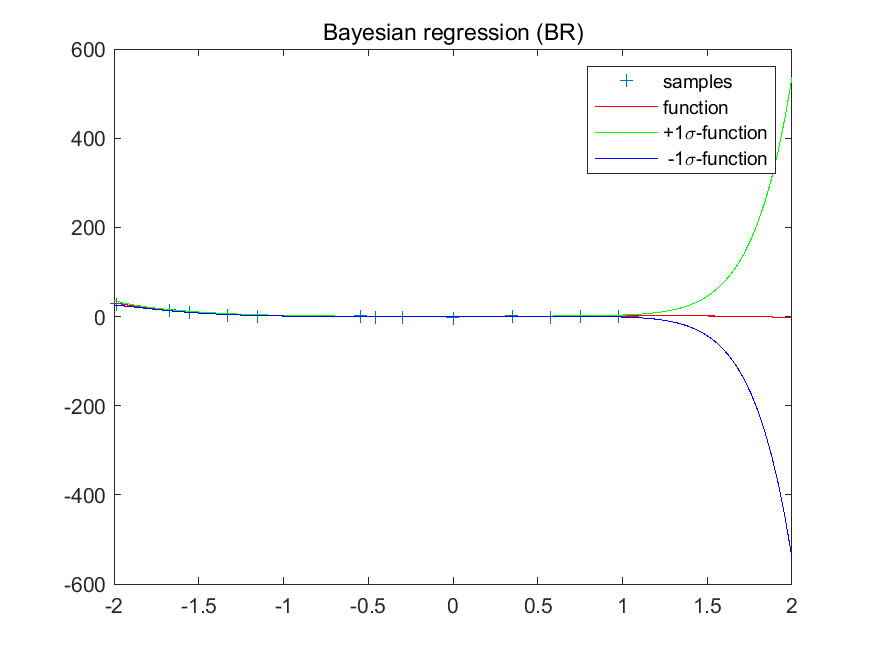
\includegraphics[width=\textwidth]{fig/1c-25-br.png} 
    \end{subfigure}
    \caption{25\% Random Sample}
\end{figure}

\begin{figure}[H]
    \centering
    \begin{subfigure}[b]{0.475\textwidth}
        \centering
        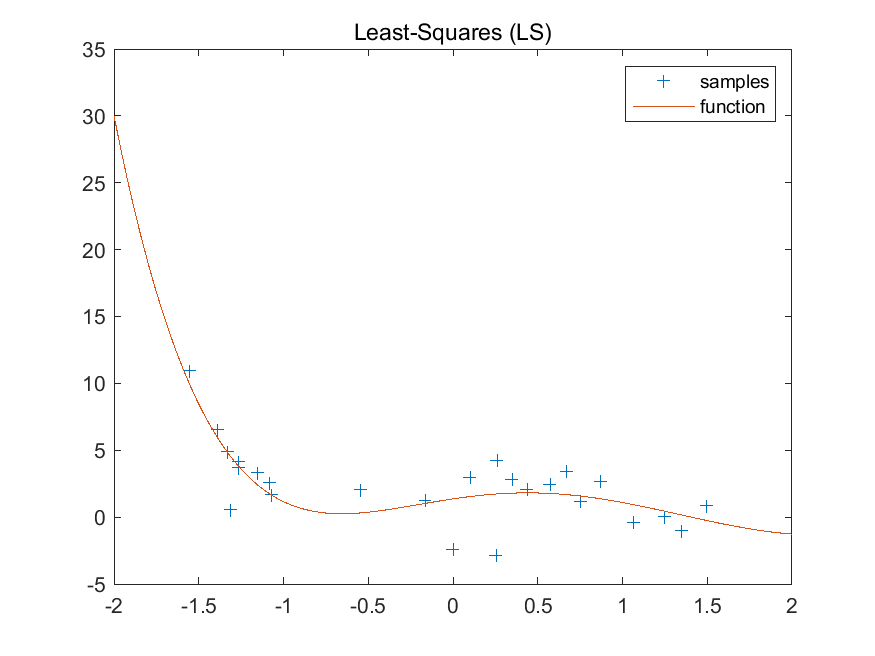
\includegraphics[width=\textwidth]{fig/1c-50-ls.png} 
    \end{subfigure}        
    \vskip\baselineskip
    \begin{subfigure}[b]{0.475\textwidth}
        \centering
        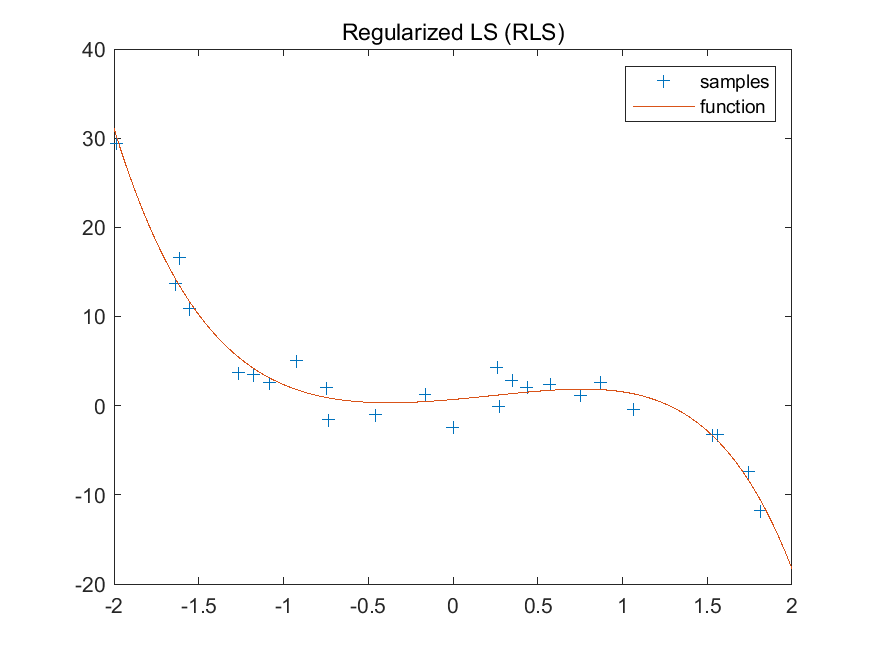
\includegraphics[width=\textwidth]{fig/1c-50-rls.png} 
    \end{subfigure}
    \hfill
    \begin{subfigure}[b]{0.475\textwidth}  
        \centering 
        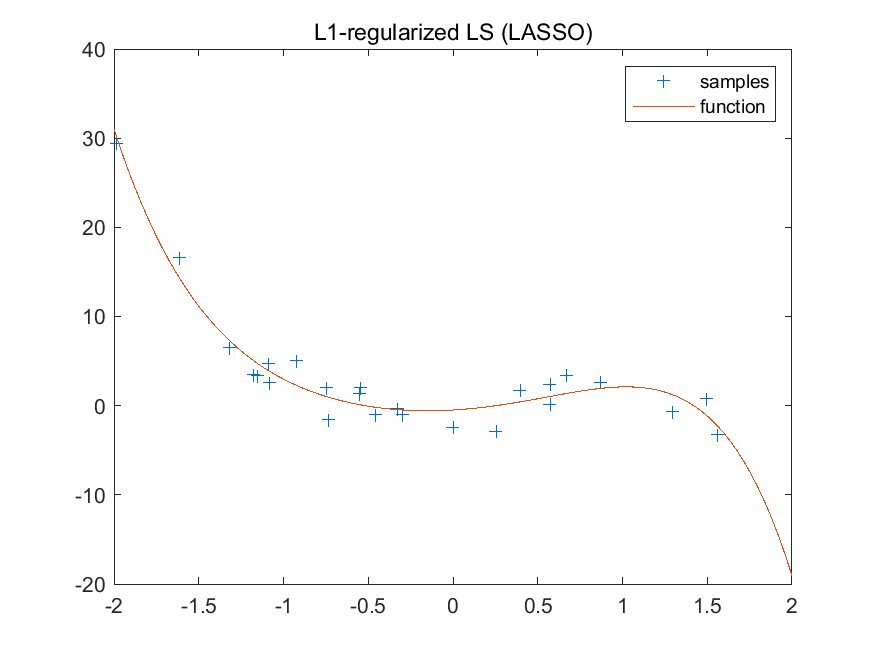
\includegraphics[width=\textwidth]{fig/1c-50-lasso.png}   
    \end{subfigure}
    \vskip\baselineskip
    \begin{subfigure}[b]{0.475\textwidth}   
        \centering 
        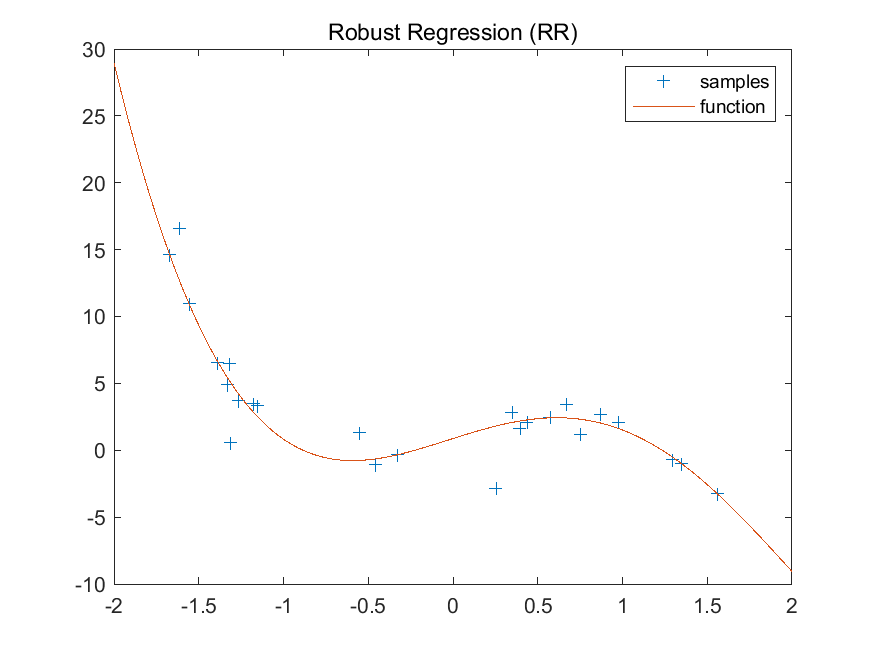
\includegraphics[width=\textwidth]{fig/1c-50-rr.png} 
    \end{subfigure}
    \quad
    \begin{subfigure}[b]{0.475\textwidth}   
        \centering 
        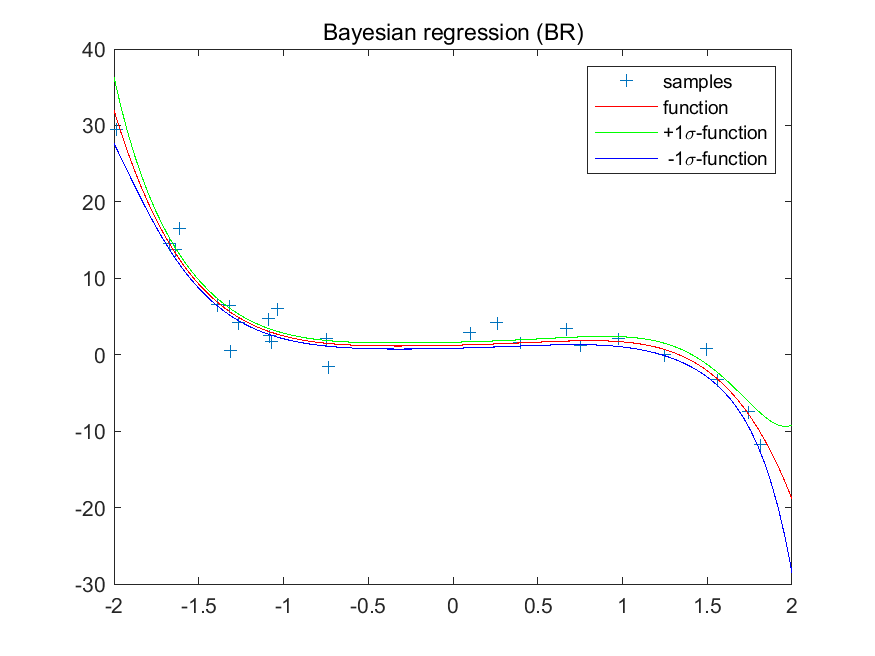
\includegraphics[width=\textwidth]{fig/1c-50-br.png} 
    \end{subfigure}
    \caption{50\% Random Sample}
\end{figure}

\begin{figure}[H]
    \centering
    \begin{subfigure}[b]{0.475\textwidth}
        \centering
        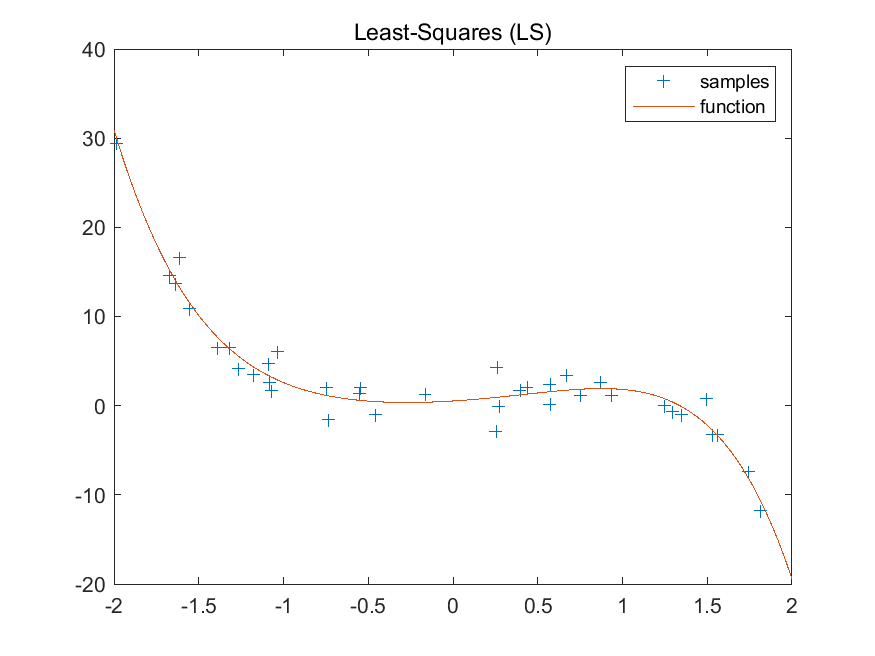
\includegraphics[width=\textwidth]{fig/1c-75-ls.png} 
    \end{subfigure}        
    \vskip\baselineskip
    \begin{subfigure}[b]{0.475\textwidth}
        \centering
        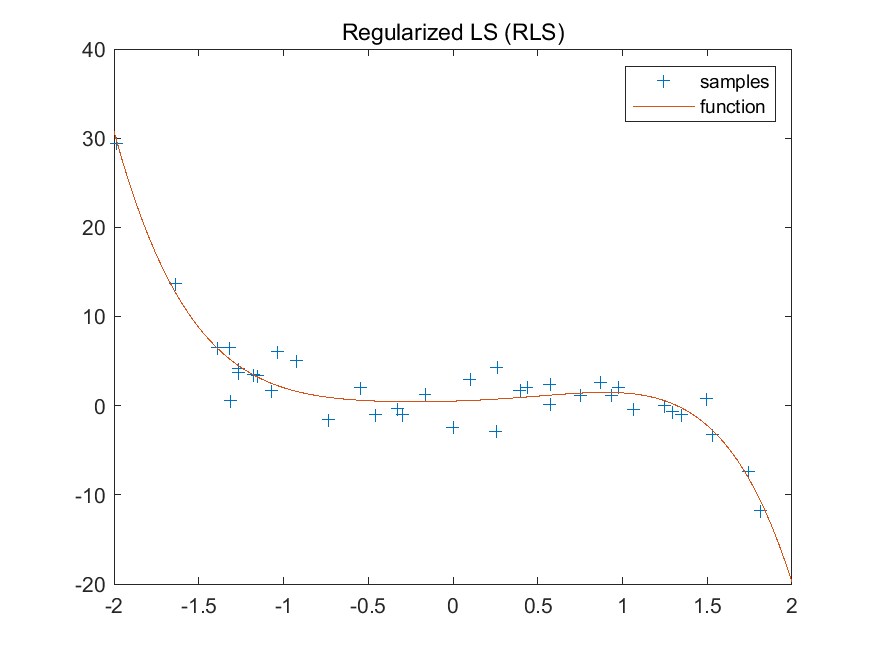
\includegraphics[width=\textwidth]{fig/1c-75-rls.png} 
    \end{subfigure}
    \hfill
    \begin{subfigure}[b]{0.475\textwidth}  
        \centering 
        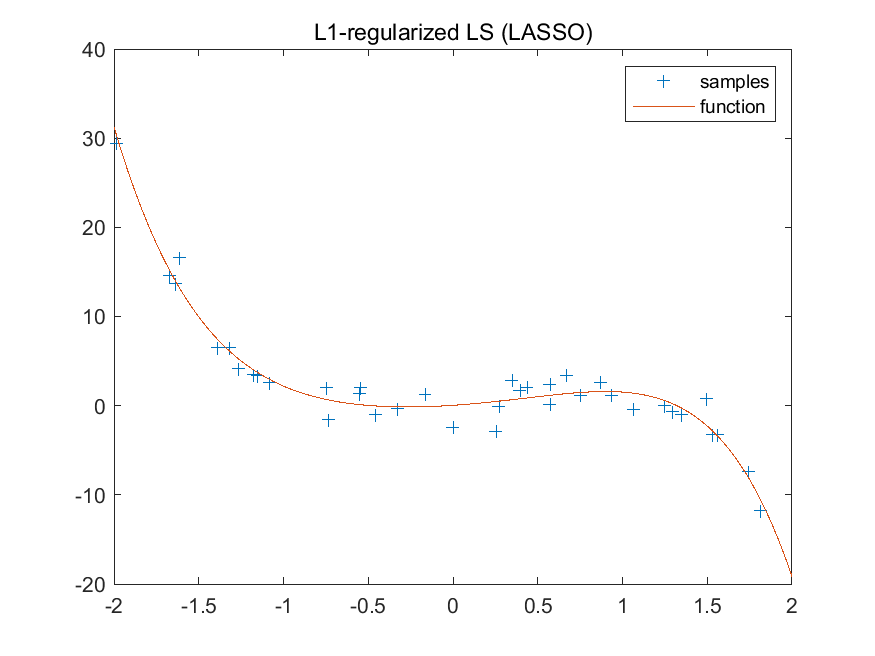
\includegraphics[width=\textwidth]{fig/1c-75-lasso.png}   
    \end{subfigure}
    \vskip\baselineskip
    \begin{subfigure}[b]{0.475\textwidth}   
        \centering 
        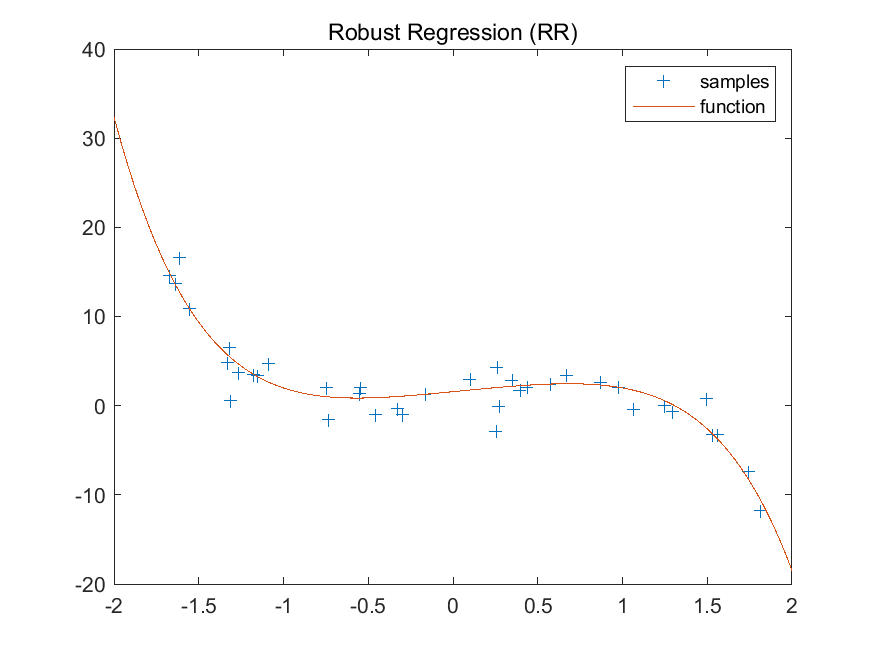
\includegraphics[width=\textwidth]{fig/1c-75-rr.png} 
    \end{subfigure}
    \quad
    \begin{subfigure}[b]{0.475\textwidth}   
        \centering 
        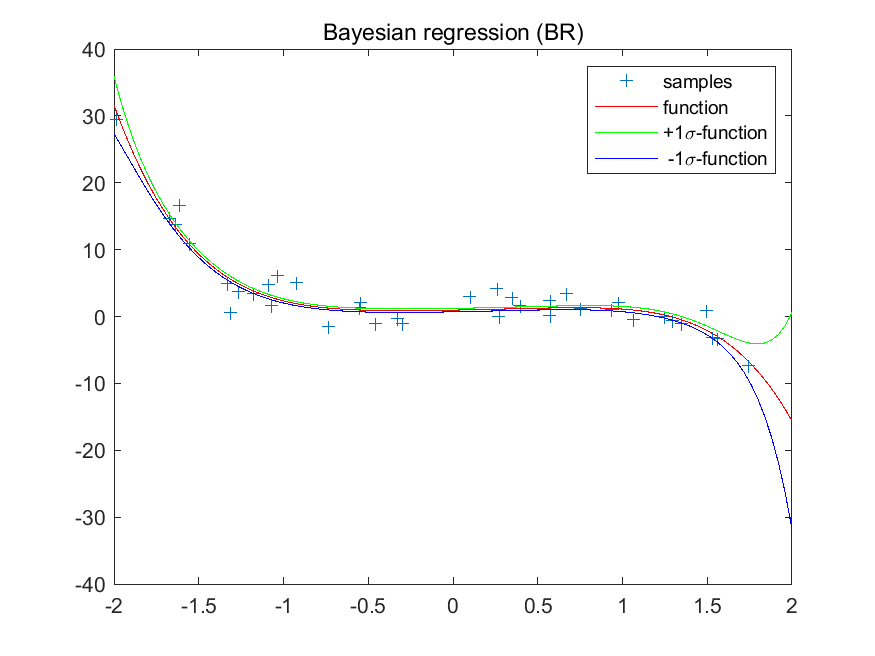
\includegraphics[width=\textwidth]{fig/1c-75-br.png} 
    \end{subfigure}
    \caption{75\% Random Sample}
\end{figure}

\subsection*{Conclusion}
Observe the experiment results, we can find that:

\begin{enumerate}[label=(\roman*)]
    \item RLS, LASSO and Bayesian Regression tends to be more robust
    \item RL and Roust Regression tends to overfit 
\end{enumerate}

\subsection*{(d) Adding Outlier Output Values}

\begin{table}[H]
    \begin{tabular}{|c|c|c|c}
    \hline
        & Least-Sqaures (LS)     & \begin{tabular}[c]{@{}c@{}}Regularized LS (RLS)\\ $\lambda$ = 0.48\end{tabular} & \multicolumn{1}{c|}{\begin{tabular}[c]{@{}c@{}}L1-Regularized LS (LASSO)\\ $\lambda$ = 1 \end{tabular}} \\ \hline
    MSE & 2.746                 & 2.352                                                                      & \multicolumn{1}{c|}{2.551}                                                                            \\ \hline
        & Robust Regression (RR) & Bayesian Regression (BR)                                                     &                                                                                                        \\ \cline{1-3}
    MSE & 0.933                 & 1.661                                                                        &                                                                                                        \\ \cline{1-3}
    \end{tabular}
\end{table}

\begin{figure}[H]
    \centering
    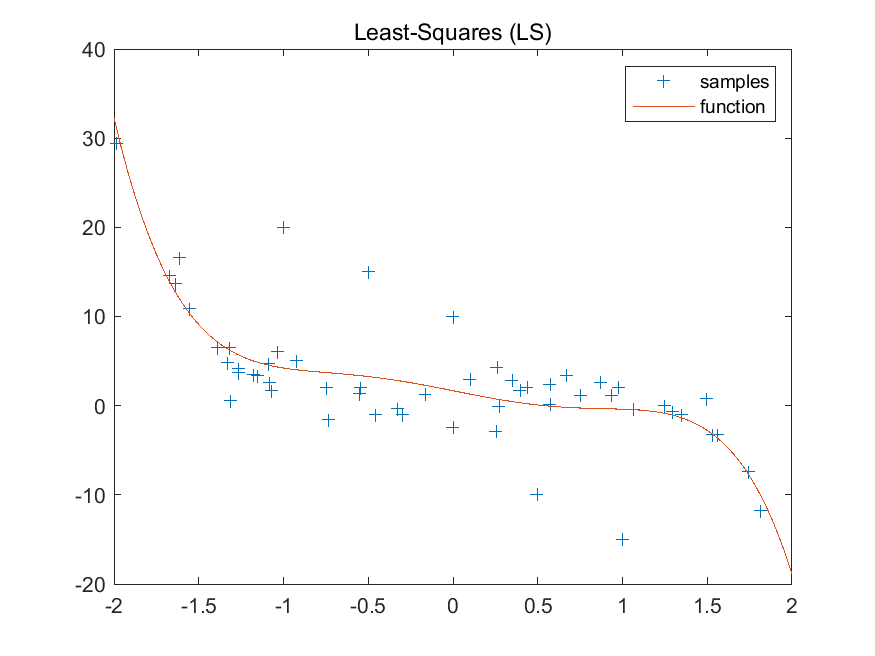
\includegraphics[width=0.6\textwidth]{fig/1d-ls.png}
    \label{fig:1b-ls}
\end{figure}

\begin{figure}[H]
    \centering
    \begin{subfigure}[b]{0.475\textwidth}
        \centering
        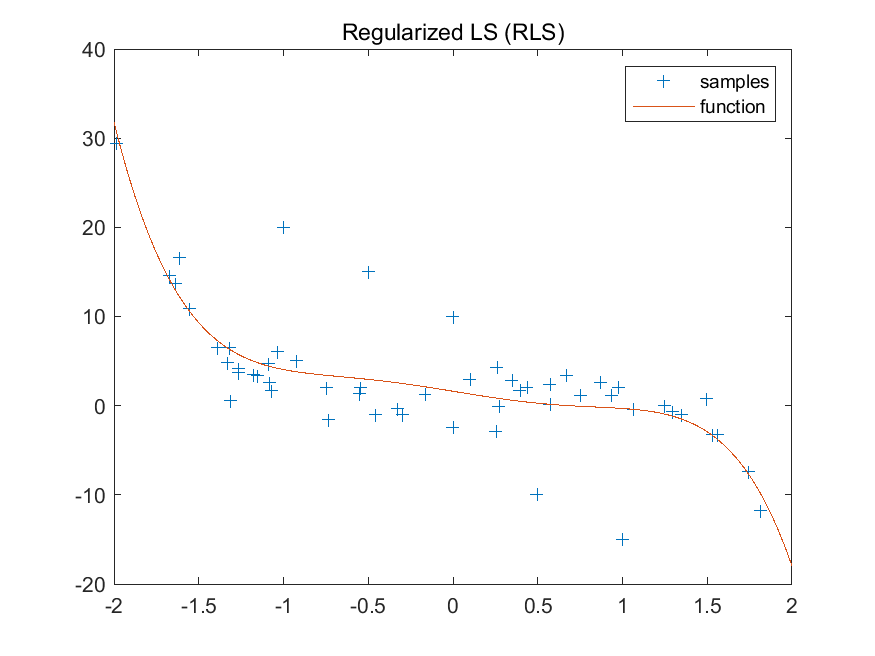
\includegraphics[width=\textwidth]{fig/1d-rls.png} 
    \end{subfigure}
    \hfill
    \begin{subfigure}[b]{0.475\textwidth}  
        \centering 
        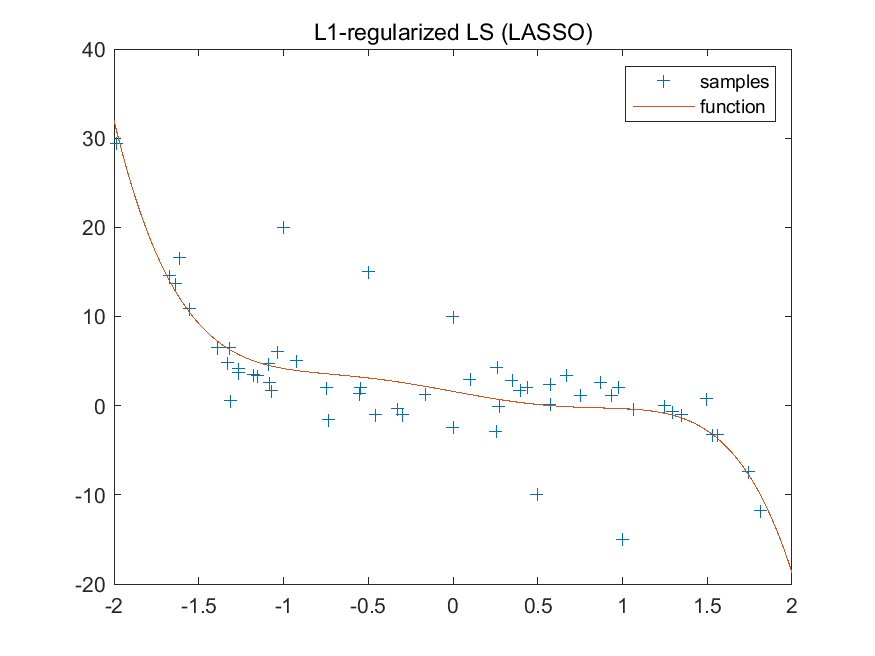
\includegraphics[width=\textwidth]{fig/1d-lasso.png}   
    \end{subfigure}
    \vskip\baselineskip
    \begin{subfigure}[b]{0.475\textwidth}   
        \centering 
        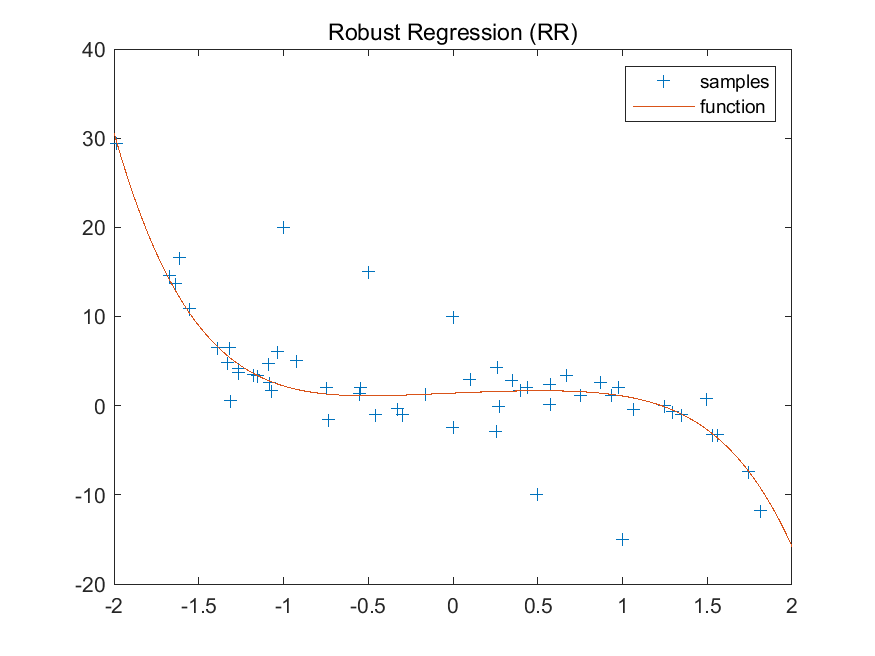
\includegraphics[width=\textwidth]{fig/1d-rr.png} 
    \end{subfigure}
    \quad
    \begin{subfigure}[b]{0.475\textwidth}   
        \centering 
        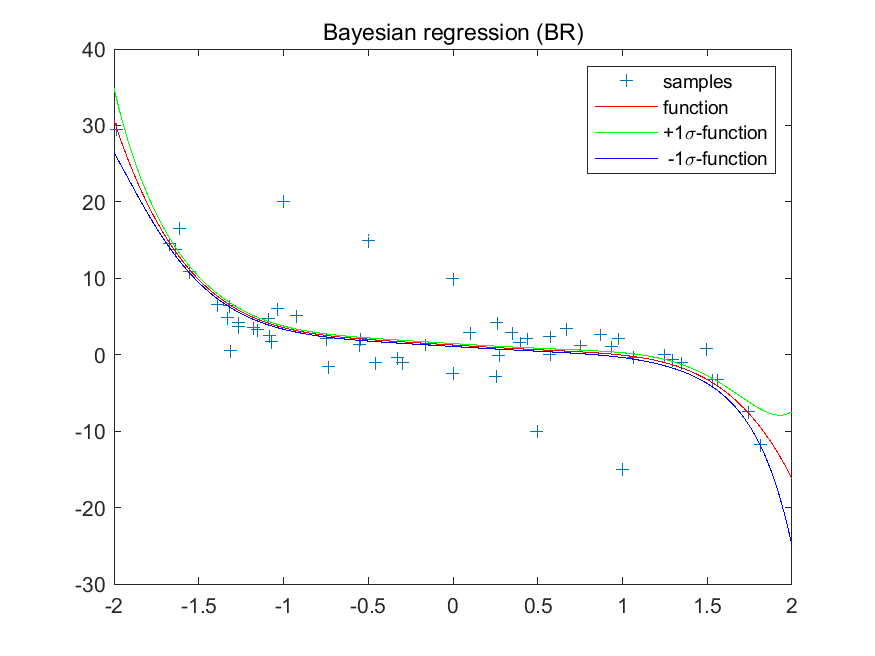
\includegraphics[width=\textwidth]{fig/1d-br.png} 
    \end{subfigure}
\end{figure}

\subsection*{Conclusion}
\begin{enumerate}[label=(\roman*)]
    \item Here, I add 5 more values, that are obviously outliers. 
    \item Robust Regression and Bayesian Regression are robust to the presence of outliers, while LS, RLS and LASSO are more sensitive
    \item Robust Regression is designed to limit the effects of outliers. Bayesian Regression contains prior knowledge which also limits the effects of data-driven prediction.
\end{enumerate}

\subsection*{(e) Higher Order Polynomial Function (10th Order)}

\begin{table}[H]
    \begin{tabular}{|c|c|c|c}
    \hline
        & Least-Sqaures (LS)     & \begin{tabular}[c]{@{}c@{}}Regularized LS (RLS)\\ $\lambda$ = 10\end{tabular} & \multicolumn{1}{c|}{\begin{tabular}[c]{@{}c@{}}L1-Regularized LS (LASSO)\\ $\lambda$ = 1.8 \end{tabular}} \\ \hline
    MSE & 7.983                & 2.877                                                                      & \multicolumn{1}{c|}{2.637}                                                                            \\ \hline
        & Robust Regression (RR) & Bayesian Regression (BR)                                                     &                                                                                                        \\ \cline{1-3}
    MSE & 1.289                 & 3.043                                                                        &                                                                                                        \\ \cline{1-3}
    \end{tabular}
\end{table}

\begin{figure}[H]
    \centering
    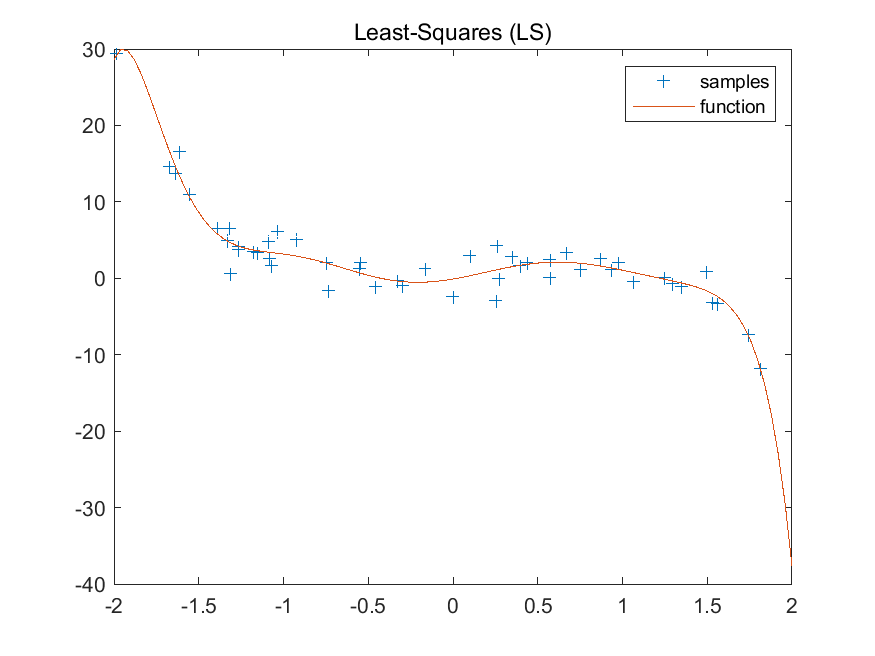
\includegraphics[width=0.6\textwidth]{fig/1e-ls.png}
    \label{fig:1b-ls}
\end{figure}

\begin{figure}[H]
    \centering
    \begin{subfigure}[b]{0.475\textwidth}
        \centering
        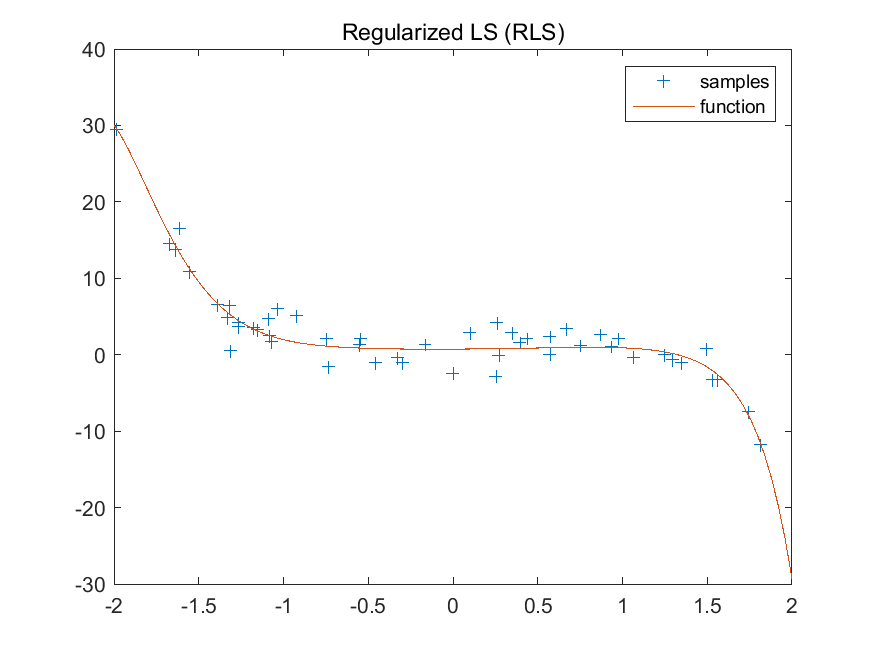
\includegraphics[width=\textwidth]{fig/1e-rls.png} 
    \end{subfigure}
    \hfill
    \begin{subfigure}[b]{0.475\textwidth}  
        \centering 
        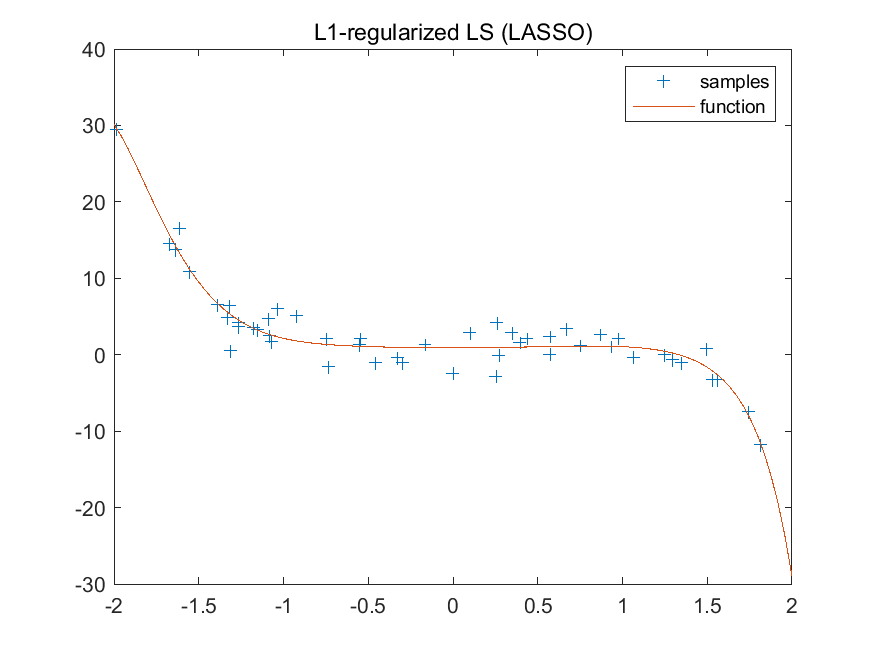
\includegraphics[width=\textwidth]{fig/1e-lasso.png}   
    \end{subfigure}
    \vskip\baselineskip
    \begin{subfigure}[b]{0.475\textwidth}   
        \centering 
        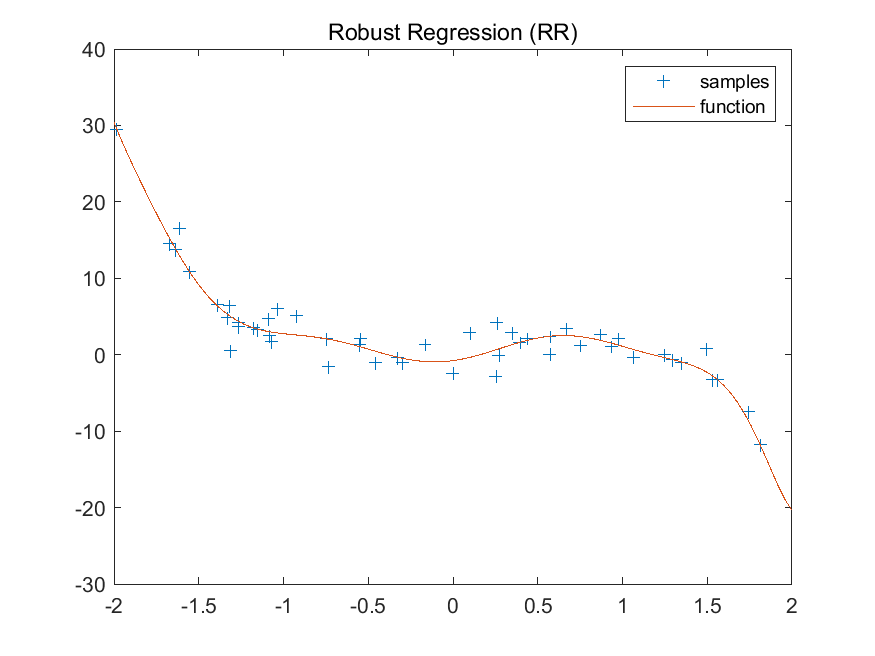
\includegraphics[width=\textwidth]{fig/1e-rr.png} 
    \end{subfigure}
    \quad
    \begin{subfigure}[b]{0.475\textwidth}   
        \centering 
        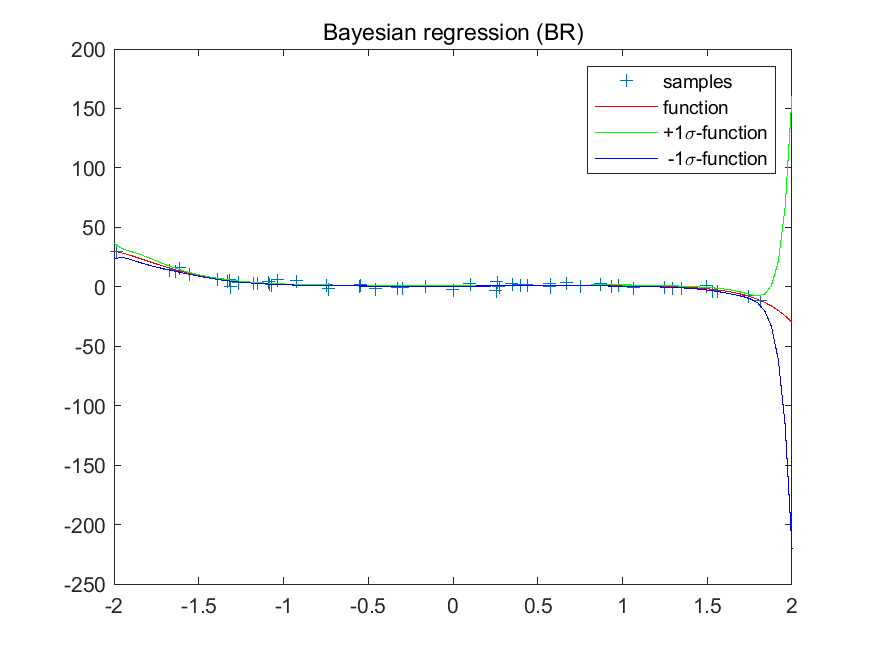
\includegraphics[width=\textwidth]{fig/1e-br.png} 
    \end{subfigure}
\end{figure}

\subsection*{Conclusion}
\begin{enumerate}[label=(\roman*)]
    \item Here, I test 10th order of polynomial function.
    \item LS tends to overfit when learning a more complex model.
    \item On the contrary, RLS and LASSO can avoid get overfitting.
\end{enumerate}

\subsection*{Codes}

Source code can be found at \url{https://github.com/yangji12138/machine-learning/tree/master/Programming%201}.

\subsubsection*{Bayesian Regression}

\lstinputlisting{../BR.m}

\subsubsection*{LASSO}

\lstinputlisting{../LASSO.m}

\subsubsection*{Linear Regression}

\lstinputlisting{../LS.m}

\subsubsection*{RLS}

\lstinputlisting{../RLS.m}

\subsubsection*{Robust Regression}

\lstinputlisting{../RR.m}

\end{document}